\documentclass{beamer}
\usepackage[utf8]{inputenc}
\usetheme{Madrid}
\usecolortheme{default}
\usepackage{amsmath,amssymb,amsfonts,amsthm}
\usepackage{txfonts}
\usepackage{tkz-euclide}
\usepackage{listings}
\usepackage{adjustbox}
\usepackage{array}
\usepackage{tabularx}
\usepackage{gvv}
\usepackage{lmodern}
\usepackage{circuitikz}
\usepackage{tikz}
\usepackage{graphicx}

\setbeamertemplate{page number in head/foot}[totalframenumber]

\usepackage{tcolorbox}
\tcbuselibrary{minted,breakable,xparse,skins}



\definecolor{bg}{gray}{0.95}
\DeclareTCBListing{mintedbox}{O{}m!O{}}{%
  breakable=true,
  listing engine=minted,
  listing only,
  minted language=#2,
  minted style=default,
  minted options={%
    linenos,
    gobble=0,
    breaklines=true,
    breakafter=,,
    fontsize=\small,
    numbersep=8pt,
    #1},
  boxsep=0pt,
  left skip=0pt,
  right skip=0pt,
  left=25pt,
  right=0pt,
  top=3pt,
  bottom=3pt,
  arc=5pt,
  leftrule=0pt,
  rightrule=0pt,
  bottomrule=2pt,
  toprule=2pt,
  colback=bg,
  colframe=orange!70,
  enhanced,
  overlay={%
    \begin{tcbclipinterior}
    \fill[orange!20!white] (frame.south west) rectangle ([xshift=20pt]frame.north west);
    \end{tcbclipinterior}},
  #3,
}
\lstset{
    language=C,
    basicstyle=\ttfamily\small,
    keywordstyle=\color{blue},
    stringstyle=\color{orange},
    commentstyle=\color{green!60!black},
    numbers=left,
    numberstyle=\tiny\color{gray},
    breaklines=true,
    showstringspaces=false,
}
%------------------------------------------------------------
%This block of code defines the information to appear in the
%Title page
\title %optional
{3.3.1}

%\subtitle{A short story}

\author % (optional)
{BALU-ai25btech11017}



\begin{document}


\frame{\titlepage}
\begin{frame}{Question}
The points \((3, 4)\) and \((2, -6)\) are situated on the \underline{\hspace{2cm}} of the line \(3x - 4y - 8 = 0\).\\ 
\end{frame}
\begin{frame}{Theoretical Solution}
Let us solve the given equation theoretically and then verify the solution computationally \\
According to the question, \\
Given two points\\
\begin{align}
\vec{a}=\begin{myvec}{3\\4}\end{myvec}\
\vec{b}=\begin{myvec}{2\\-6}\end{myvec}\
\end{align}
\begin{align}
\vec{n}=\begin{myvec}{\frac{-3}{4}\\1}\end{myvec}
\end{align}
Equation of line is
\begin{align}
    \vec{n}^T\vec{x}=1
\end{align}
\end{frame}
\begin{frame}{Theoretical Solution}
\begin{align}
    \vec{n}^T\vec{a}-1=\frac{3}{4}\\
    \vec{n}^T\vec{b}-1=\frac{-17}{2}
\end{align}
As the values are in opposite sign the points are situated in opposite direction w.r.t line
\end{frame}
\begin{frame}[fragile]
    \frametitle{C Code}

    \begin{lstlisting}
#include <stdio.h>

int main() {
    // Line: 3x - 4y - 8 = 0
    // Points
    int x1 = 3, y1 = 4;
    int x2 = 2, y2 = -6;

    // Evaluate f(x,y) = 3x - 4y - 8
    int f1 = 3*x1 - 4*y1 - 8;
    int f2 = 3*x2 - 4*y2 - 8;

    printf("Line equation: 3x - 4y - 8 = 0\n");

    printf("For point (3,4), f(x,y) = %d -> ", f1);
    if(f1 == 0) printf("Point lies on the line.\n");
    else if(f1 > 0) printf("Point lies on one side of the line.\n");
    else printf("Point lies on the other side of the line.\n");

   

     \end{lstlisting}
\end{frame}
\begin{frame}[fragile]
    \frametitle{C Code - Resultant velocity}
    \begin{lstlisting}
  printf("For point (2,-6), f(x,y) = %d -> ", f2);
    if(f2 == 0) printf("Point lies on the line.\n");
    else if(f2 > 0) printf("Point lies on the same side as (3,4).\n");
    else printf("Point lies on the opposite side of (3,4).\n");

    // Final answer
    if ((f1 > 0 && f2 > 0) || (f1 < 0 && f2 < 0)) {
        printf("\nBoth points are on the SAME side of the line.\n");
    } else if (f1 == 0 || f2 == 0) {
        printf("\nOne of the points lies on the line.\n");
    } else {
        printf("\nThe points are on OPPOSITE sides of the line.\n");
    }

    return 0;
}
    \end{lstlisting}
\end{frame}
\begin{frame}[fragile]
    \frametitle{Python Code}
    \begin{lstlisting}
import numpy as np
import matplotlib.pyplot as plt

# Define the line 3x - 4y - 8 = 0  =>  y = (3x - 8)/4
x = np.linspace(-2, 6, 400)
y = (3*x - 8)/4

# Points
points = [(3, 4), (2, -6)]

# Plot line
plt.plot(x, y, 'b', label='3x - 4y - 8 = 0')

# Plot points
for px, py in points:
    plt.plot(px, py, 'ro')
    plt.text(px+0.2, py, f"({px},{py})", fontsize=10)





    \end{lstlisting}
\end{frame}

\begin{frame}[fragile]
    \frametitle{Python Code}
    \begin{lstlisting}
# Formatting
plt.axhline(0, color='black', linewidth=0.5)
plt.axvline(0, color='black', linewidth=0.5)
plt.grid(True, linestyle='--', alpha=0.6)
plt.xlabel("x")
plt.ylabel("y")
plt.legend()
plt.title("Line and Points")

# Save figure
plt.savefig("line_points.png", dpi=300)
plt.show()
    \end{lstlisting}
\end{frame}
\begin{frame}{Plot}
    \centering
    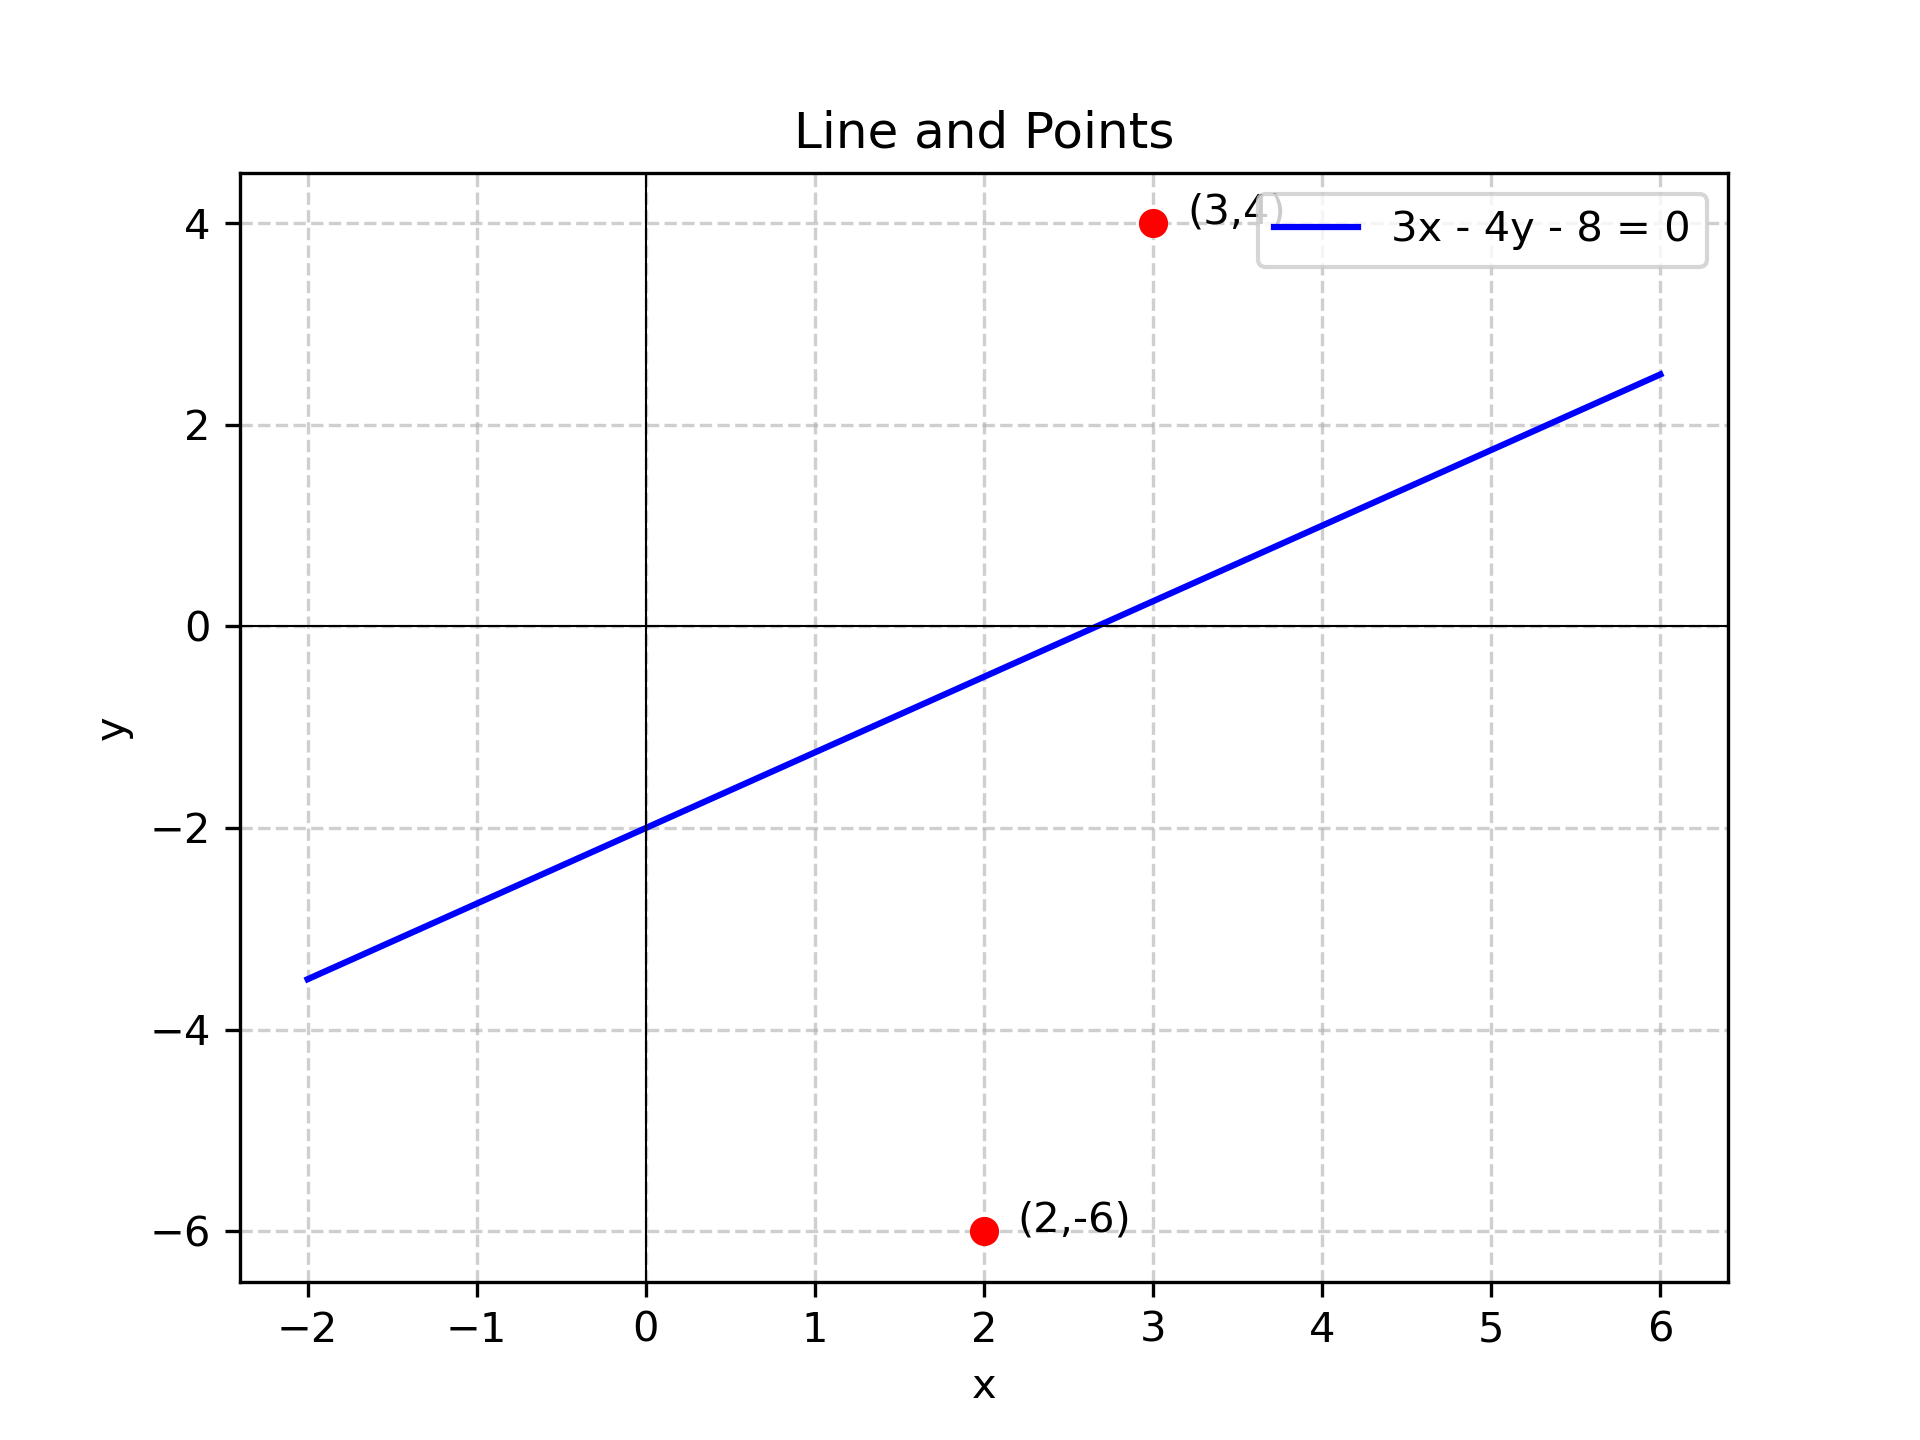
\includegraphics[width=\columnwidth, height=0.8\textheight, keepaspectratio]{figs/line_points.png}     
\end{frame}




\end{document}